\chapter{Experimental Apparatus}
\label{chap:Exp}

\indent The study of standard model (SM) physics at the TeV scale and search for potentially new physics beyond the standard model (BSM) is the highlight of current physics programs at the Large Hadron Collider (LHC).  The LHC is a circular superconductor hadron-hadron accelerator capable of accelerating and colliding both protons and lead ions.  The LHC is built in the previous LEP tunnels between 45 to 170m underground near the city of Geneva at the Organization for European Nuclear Research or CERN. \\

\indent During 2015 to 2016, the LHC collided protons with a center of mass energy of $\sqrt{13}$ TeV.  The LHC has already surpassed its design peak instantaneous luminosity by reach peak instantaneous luminosities of $1.34 \times 10^{34}$ cm$^{-2}$ sec$^{-1}$.  \\

\indent The LHC use 4 major particle detectors located at its 4 interaction points to study the result of these collisions.  Two of these, ATLAS and CMS are hermitic $4\pi$ general purpose detectors that study a wide variety of SM and BSM physics including SUSY.  ATLAS and CMS are located at the opposite end of the ring to ensure equal luminosity and serve as validations to one another.  The ALICE detector specializes in collisions of heavy ions. LHCb specializes in physics involving the bottom quark. \\

\indent In addition to the 4 major particle detectors, three smaller experiments, TOTEM, MoEDAL and LHCf, study proton proton scattering cross sections, diffractive processes, and cosmic ray physics.  ~\\

\indent This analysis uses data collected by the ATLAS detector in 2015 and 2016.  A summary of the LHC accelerator complex and the ATLAS detector will be given in this chapter. \\

\section{The CERN Accelerator Complex and the Large Hadron Collider}

\indent Before collision in one of the LHC experiments, protons are first accelerated through a series of accelerators that form the CERN accelerator complex shown in figure \ref{LHC:fig:LHCComplex}.  Hydrogen atoms are ionized and the resulting protons are first accelerated to $50 \mev$ by the Linear Accelerator 2 (LINAC2).  Then the protons are injected into a series of circular accelerators, the Proton Synchrotron Booster (PSB), the Proton Synchrotron (PS) and Super Proton Synchrotron (SPS) which further increases the proton energy to 1.4, 25 and 450 GeV respectively.  The protons are arranged into bunches composed of approximately $1.1 \times 10^{11}$ protons each and injected into the LHC.  During 2015 and 2016, the LHC operated with both 50 ns and 25 bunch spacings and can nominally accommodate up to 2808 bunches in a single run. \\

\begin{figure}[h!]
%\begin{center}
\centering
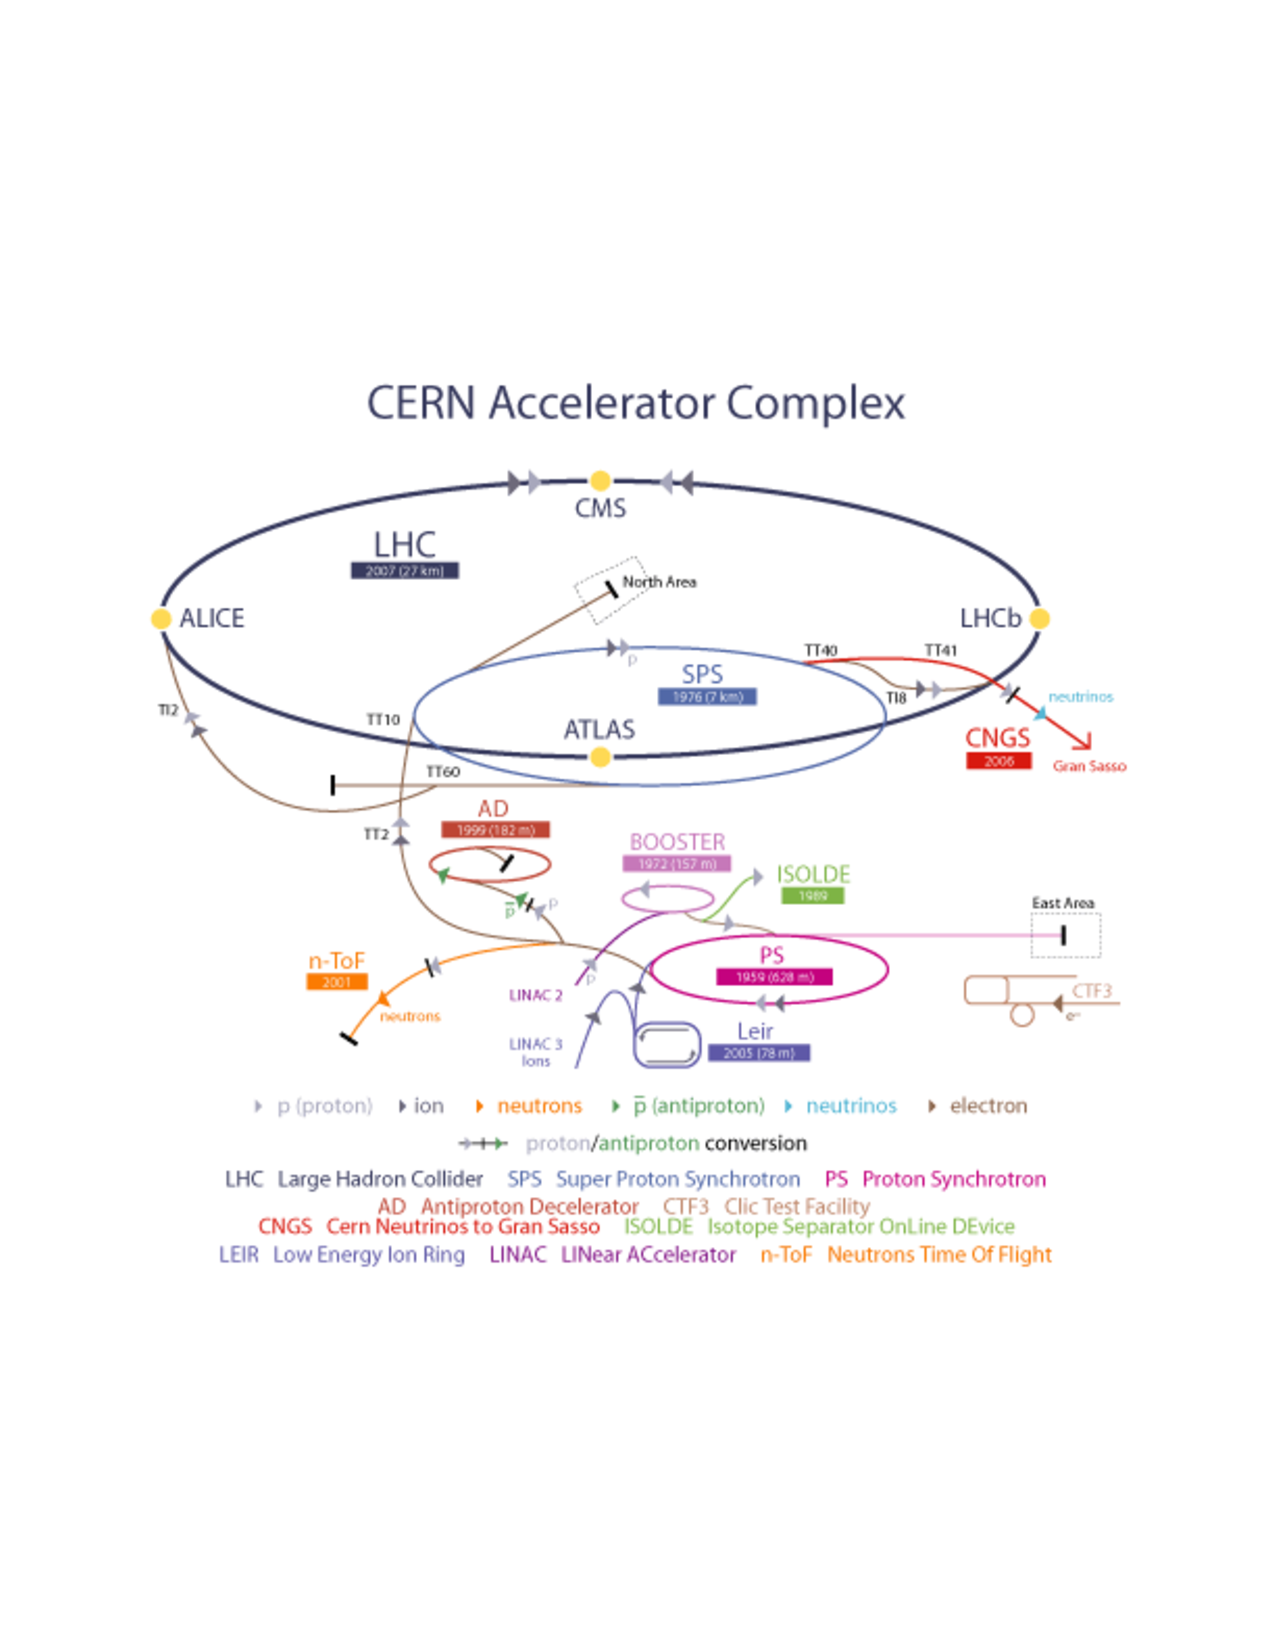
\includegraphics[width=0.65\textwidth, angle=0]{figures/LHC_ATLAS/AccComplex0700829.pdf}
\caption{ The Large Hadron Collider complex. (Taken from \cite{LHC}) \label{LHC:fig:LHCComplex}}
%\end{center}
\end{figure}

\indent The LHC shares the same geometry as LEP with eight arc and eight straight sections.  The main LHC body consist of 1232 dipole Niobium Titanium superconducting magnets that are used to generate the 8.33 Tesla magnetic field necessary to bend the 7 TeV proton beams.  The LHC uses a {\tt two-in-one} magnet design shown in figure \ref{LHC_Xsec} both as a cost saving measure and because of the limited space in the tunnels. The two-in-one magnet design uses a single cryogenic system and vacuum vessel for both proton beams.  \\

\begin{figure}[h!]
%\begin{center}
\centering
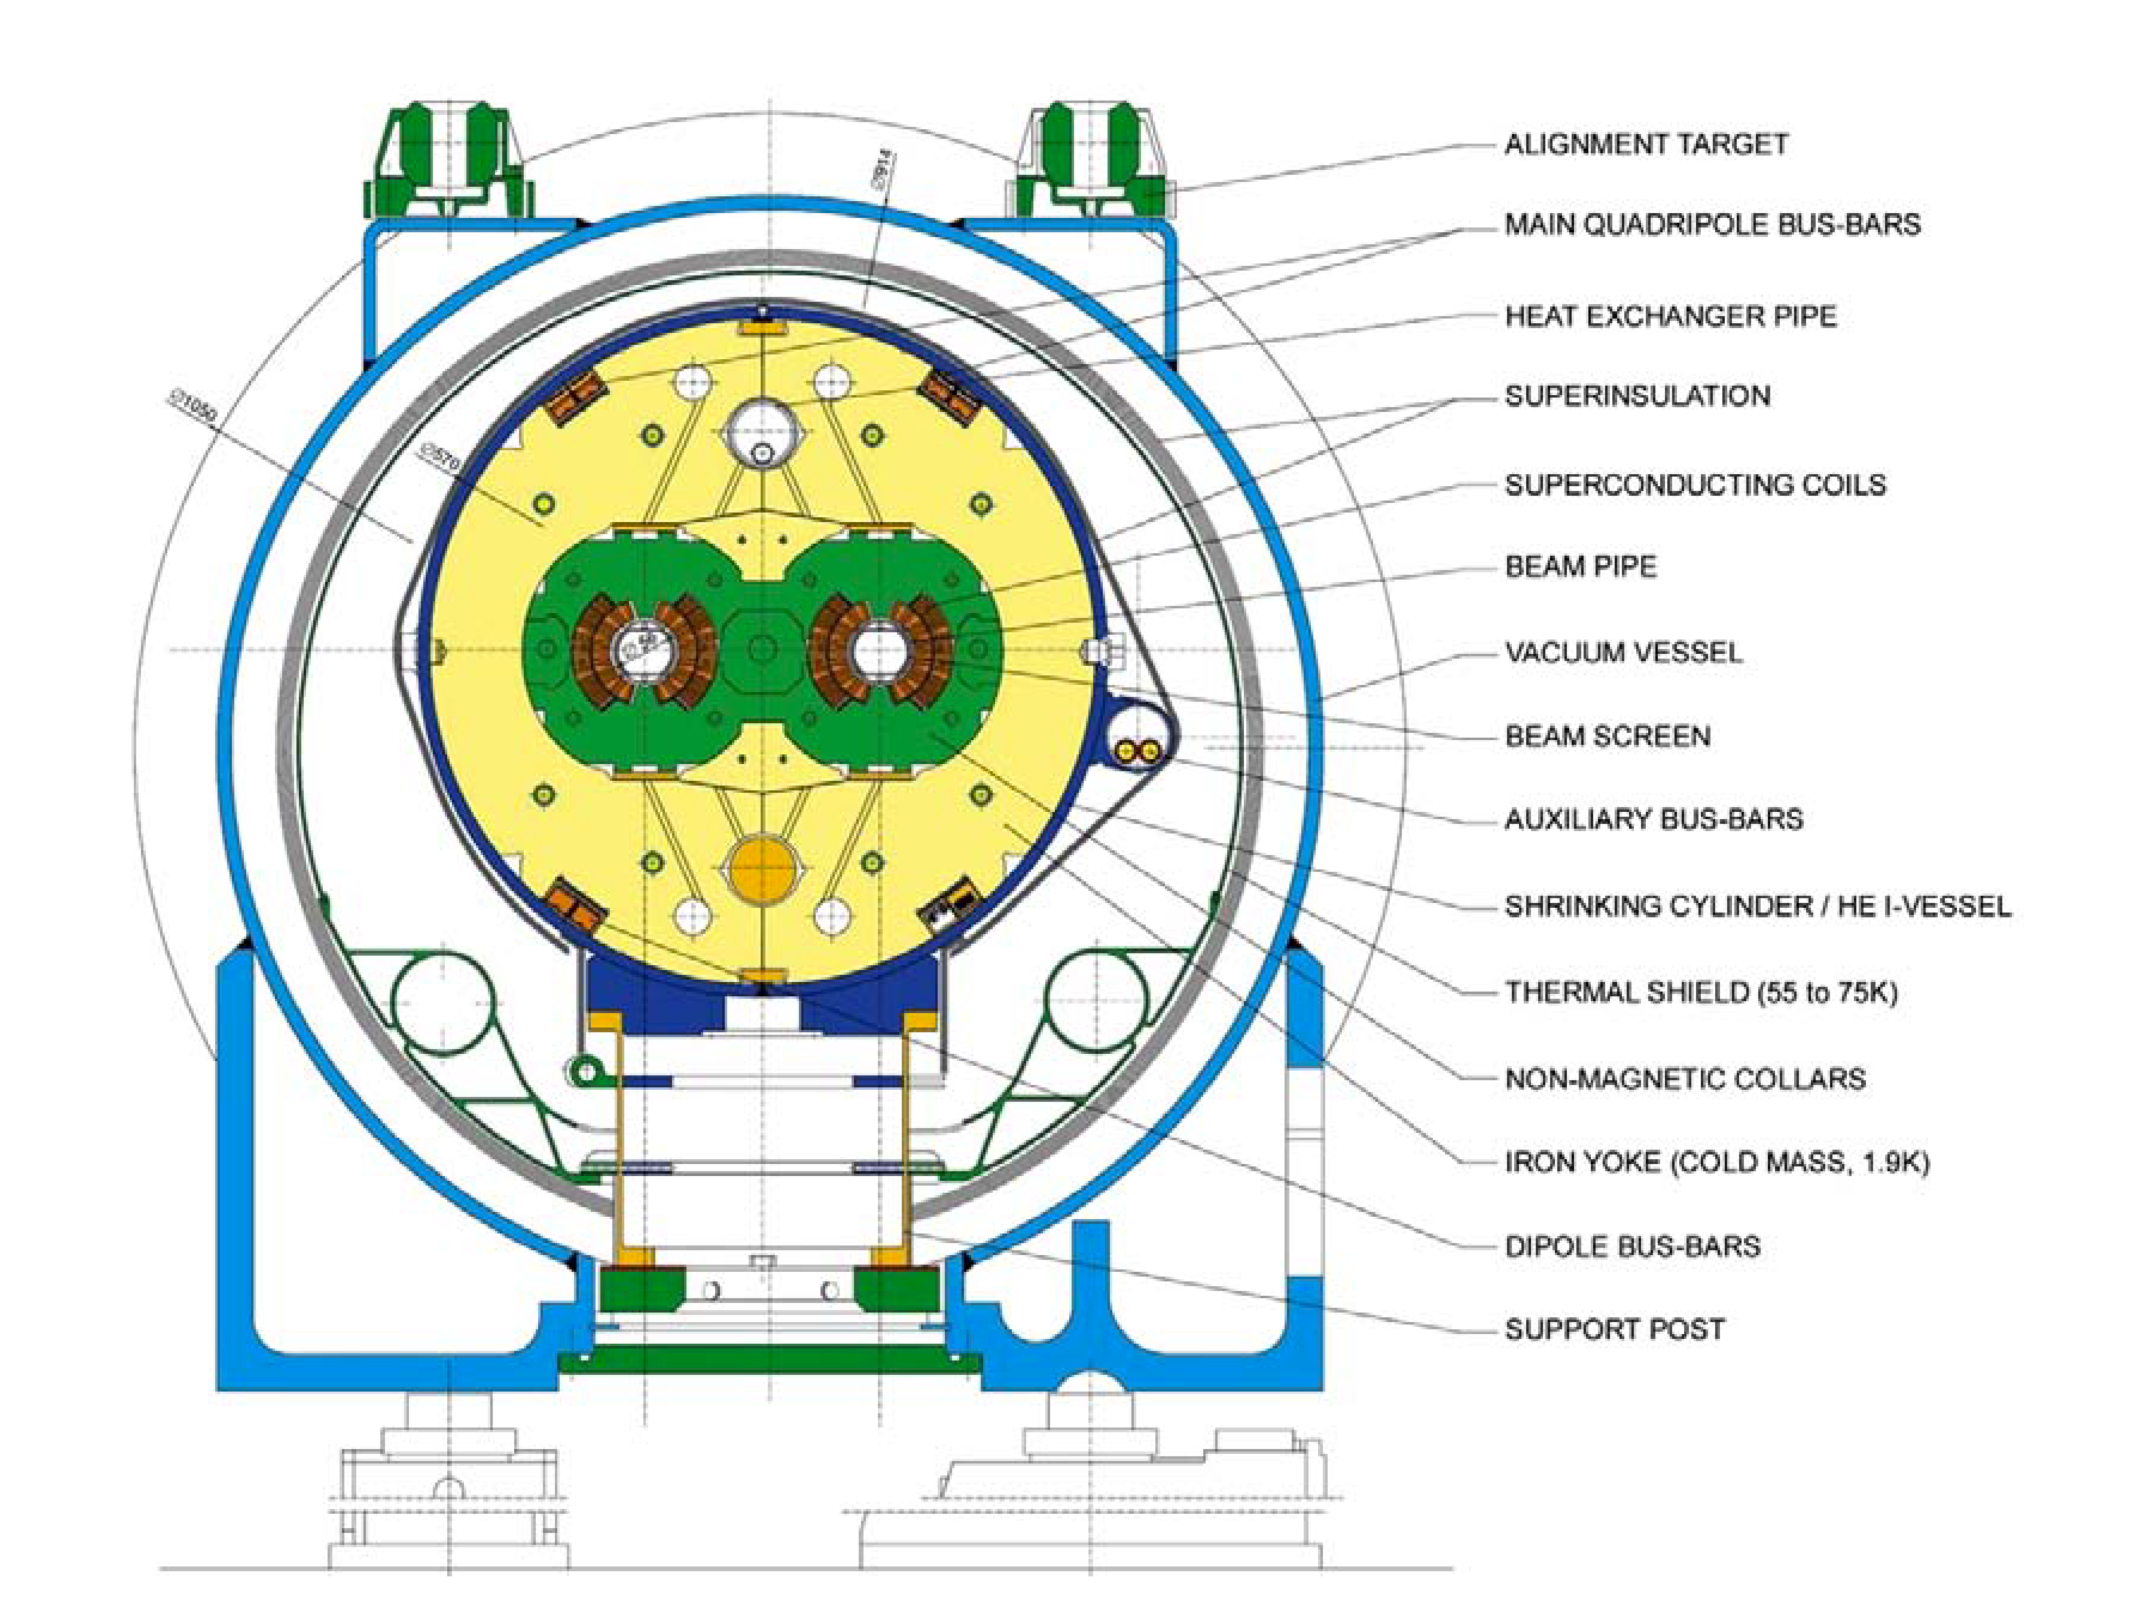
\includegraphics[width=0.75\textwidth]{figures/LHC_ATLAS/LHCCrossSection.pdf}
\caption{ Cross-Sectional View of a Large Hadron Collider Dipole Magnet. Figure taken from \cite{LHC} }
 \label{LHC_Xsec}
%\end{center}
\end{figure}

\indent  392 quadruple magnets are placed after approximately every three dipole sections to stabilize and focus the beam using the principle of strong focusing.  Higher order sextupoles and octupoles magnets provide further corrections. \\

\indent The beams are accelerated using a 400 MHz superconducting radio frequency (RF) cavity system.  Two independent RF systems are used for the two beams heading in opposite directions.  Each RF system consist of eight cavities.  The total accelerating field inside the cavity is 5 MV/m and each cavity delivers 2 MV of accelerating voltage.  The beams are bent back to repeatedly receive acceleration via the same cavity.  \\

\indent Further upgrades planed in the Phase 1 shutdown between 2019 and 2021 are projected to further double the instantaneous luminosity and allow the LHC to reach its designed center of mass collision energy of $\sqrt{14} \tev$. \cite{Phase1} \\

\section{The ATLAS Detector}
\label{LHC:detector}

\indent The ATLAS Detector shown in figure \ref{LHC:fig:ATLASDet} is a general purpose detector that is designed to both search for new physics at the TeV scale and precision measurement of SM parameters.\cite{ATLAS_JINST}  The ATLAS detector is composed of several subdetector arranged layer by layer in concentric cylinders surrounding the interaction point.  The hermitic detector cover nearly the entire $4\pi$ solid angle around the interaction point. \\

\begin{figure}[h!]
%\begin{center}
\centering
\includegraphics[width=0.75\textwidth, angle=0]{figures/LHC_ATLAS/ATLAS_SE_Corrected7.eps}
\caption{ Cutaway view of the ATLAS detector with different sub-detector systems labeled. Figure taken from \cite{ATLAS_JINST} \label{LHC:fig:ATLASDet}}
%\end{center}
\end{figure}

\indent Each subdetector system specialize in the detection of a specific subset of particles that are expected to result from collisions provided by the LHC.  Starting from the interaction point and moving out, the detector can be divided into the inner tracker, the electromagnetic calorimeter, the hadronic calorimeter and the muon spectrometer.  The detector signatures left by different particles can be seen in figure \ref{LHC:fig:ATLASSig}. \\

\begin{figure}[h!]
%\begin{center}
\centering
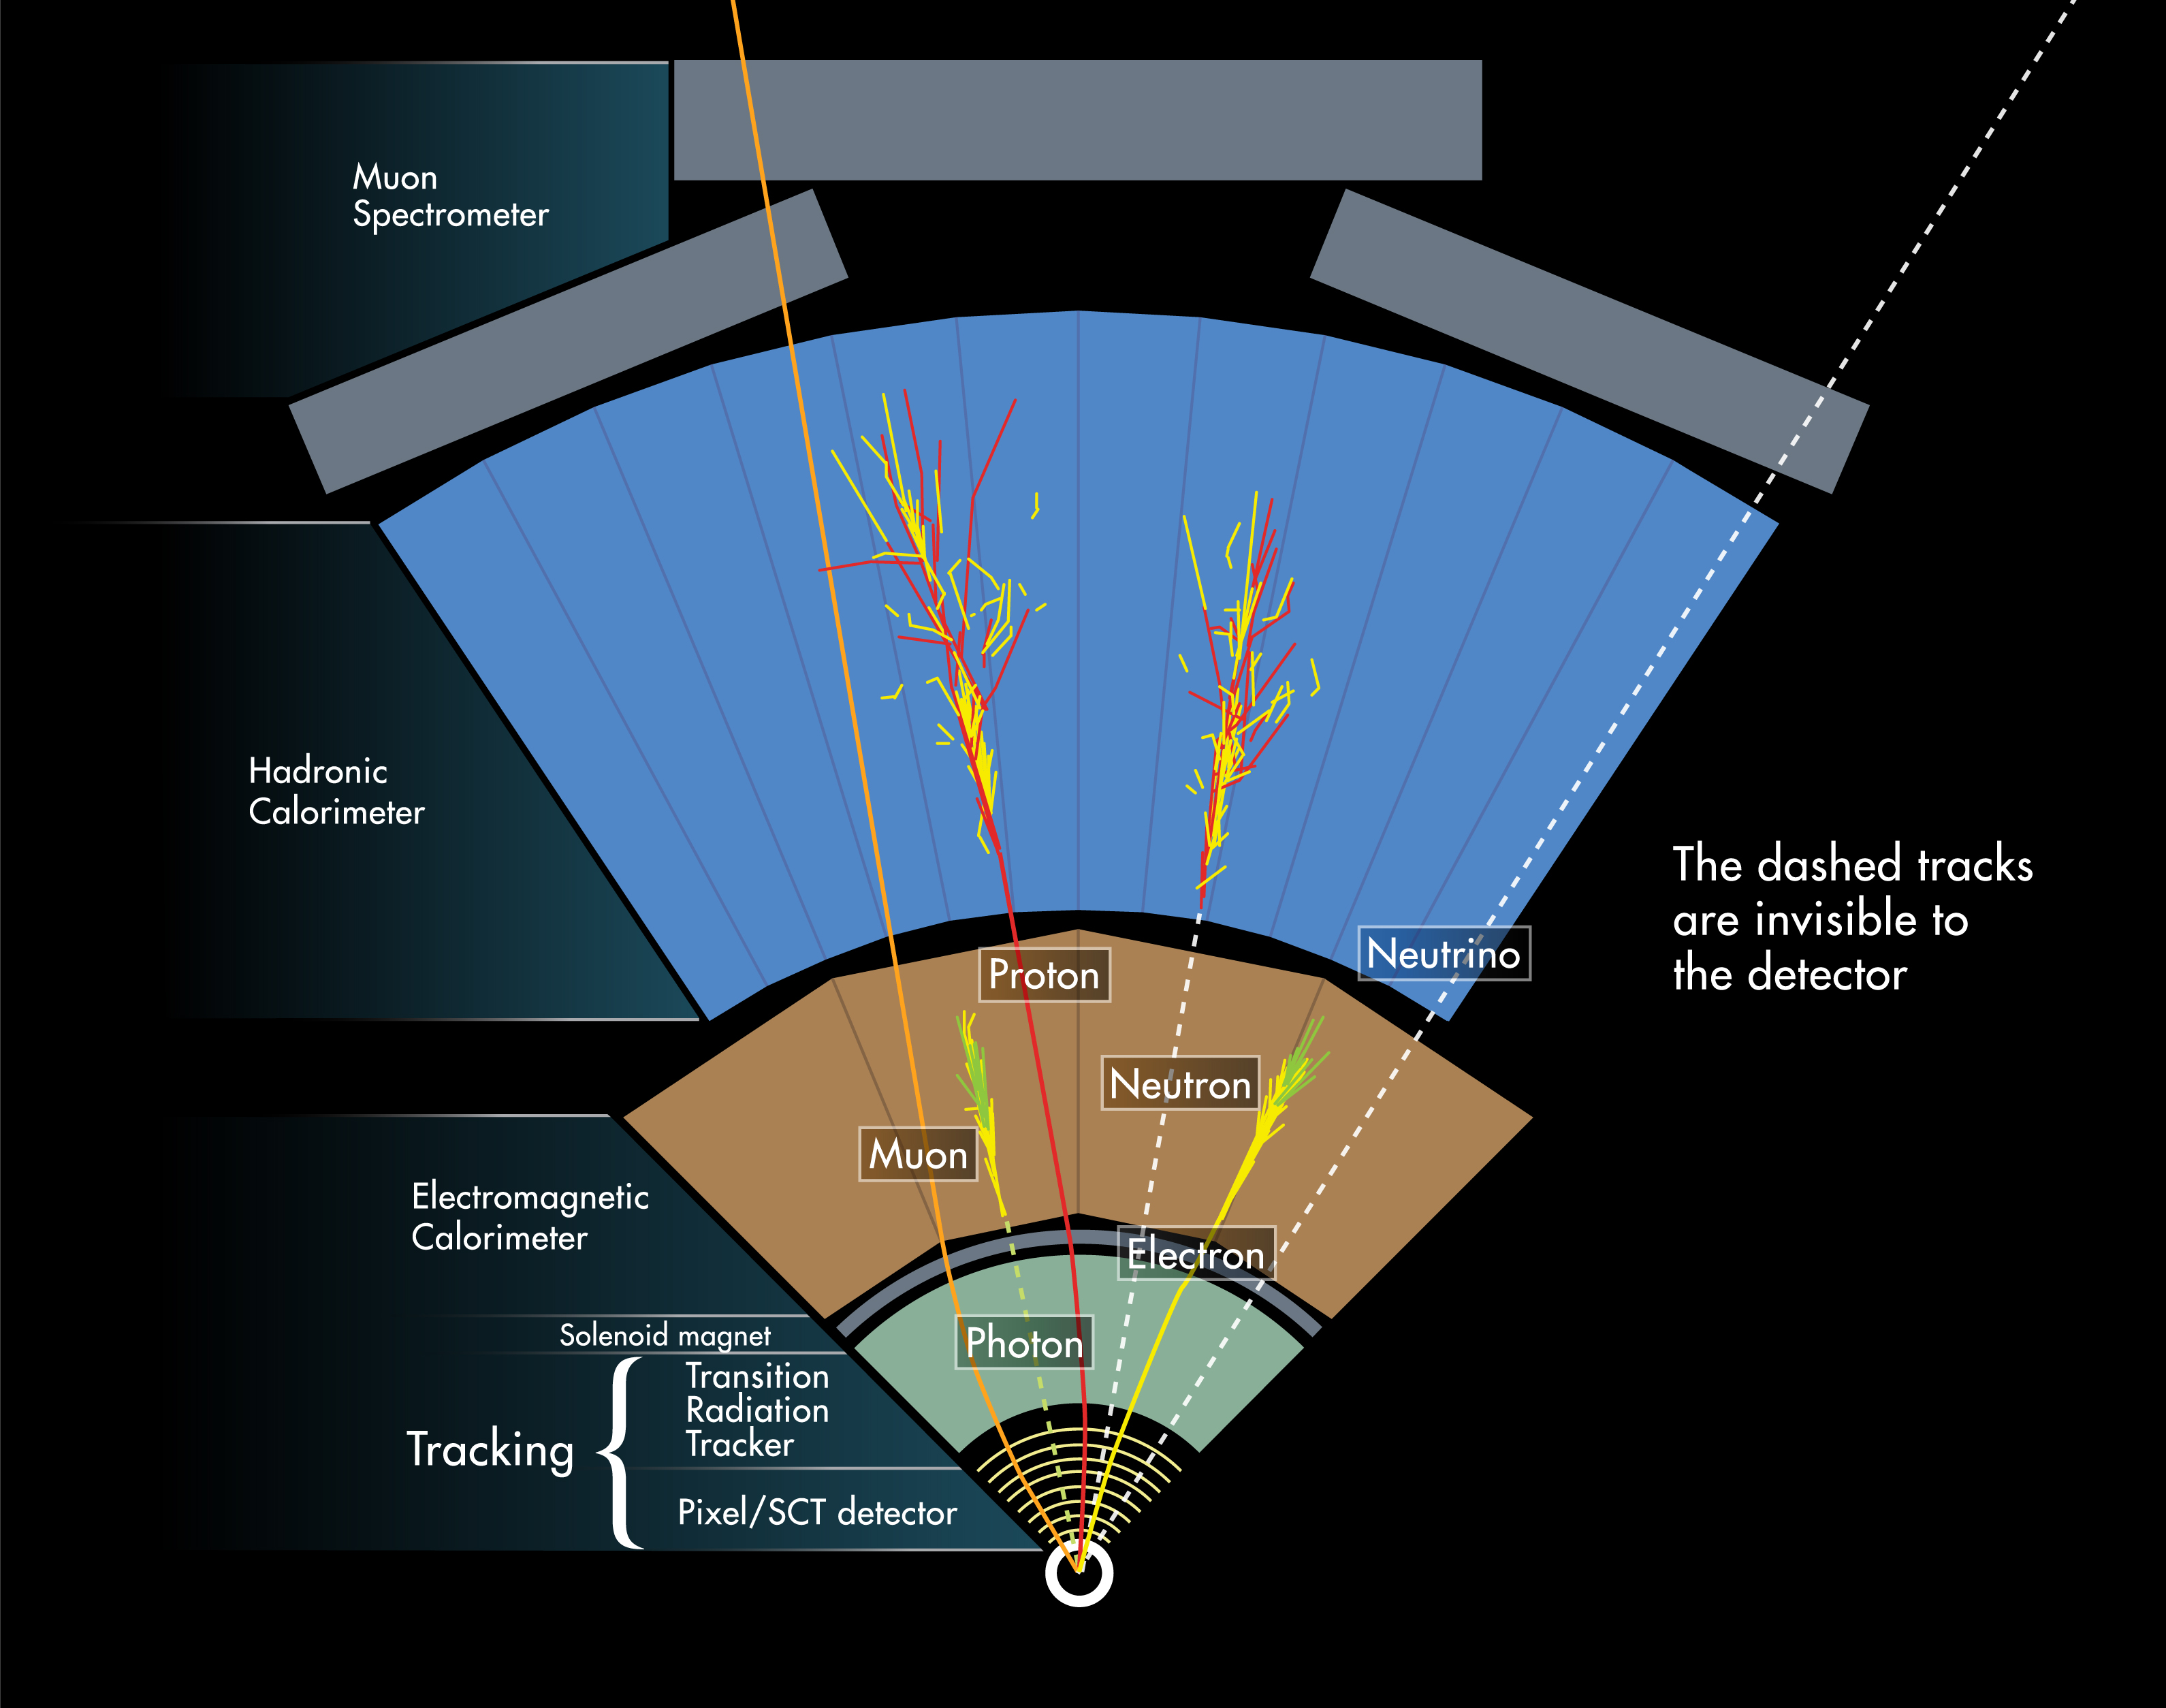
\includegraphics[width=0.65\textwidth, angle=0]{figures/LHC_ATLAS/ATLAS_Signature.jpg}
\caption{ Artistic representation of different detector signatures left by particles in ATLAS. Figure taken from \cite{ATLASSig} \label{LHC:fig:ATLASSig}}
%\end{center}
\end{figure}

\indent Details on the reconstruction of physics objects can be found in chapter \ref{chap:reco}.  A brief description of detector signatures will be given here in order to motivate the purpose of each subdetector system. \\

\indent The inner tracker measure the position of charged particles as they fly through the detector.  These positions measurements are then connected to form a track that follows the flight path of the charged particle.  A 2 Tesla axial magnetic field bath the inner detector volume and is provide by the central solenoid superconducting magnet.  The magnetic field bends any charged particle in the inner tracker.  The momenta of the charged particle can be identified by the amount of bend in the track relative to the particle charge and mass.  \\

\indent The calorimeters measure the energy of all charged and neutral particles that interact via the electromagnetic and strong force.  The particle interact with the dense absorbing material via a number of interactions.  The dominant interaction for electromagnetically charged particles such as the electron is photon emission through bremsstrahlung and ionization.  Neutral high energy photons interact primarily by pair producing electrons.  Any emitted photon and electron will pair produce electrons emit photon until the resulting particles no longer have enough energy to continue the process.  This cascade of particles is called a particle shower.  Hadronic particles that interact via the strong force will also form analogous hadronic showers.  \\

\indent The shower particles deposit energy in the layers of the calorimeter with an {\it active} material.  The number of shower particles are then measured by the active material resulting in a signal.  The ATLAS calorimeter alternates between absorber and active material layers.  Thereby measuring the longitudinal and lateral shower shape and shower depth by combining information from the different layers. Showers from electromagnetic objects such as photons and electrons form denser narrow profiles while showers from strongly interacting particles form board showers that penetrate deep into the hadronic calorimeter. \\

\indent Muons are the only charged SM particle that are expected to be able to fully penetrate the calorimeter in-tact.  They in turn leave a track in the muon spectrometer.  This track can be matched to the inner detector track forming a combined muon track that traverses the entire detector.  A set of barrel and endcap toroid magnets provide the magnetic field to the muon spectrometer and adding to the momenta measurement of muons.  Fields vary depending on location but on average an integrated field of 2.5 $T \dot m$ and 4 $T \dot m$ are expected for muons traversing through the barrel and endcap.\\

\indent The combination of these different detector signatures is combined to identify and reconstruct the many different particles produced in a particle collision.  Electrons leave an electromagnetic shower in the calorimeter with an associated track.  Unconverted photons leave an electromagnetic shower without an associated track.  Hadrons fragment into jets and leave a hadronic shower in both the inner detector and hadronic calorimeter with perhaps a number of associated ID tracks.  Muons are reconstructed from a combined ID and MS track with limited energy deposited in the calorimeter.  Taus either decay leptonically or semileptonically to an electron or muon or decays hadronically to pions and leave a narrow hadronic shower in the calorimeter with one or three associated tracks.  Particles that interact via only the weak force i.e. neutrinos do not interact with the ATLAS detector.  They escape the detector completely and their presence are inferred through the conservation of transverse momenta.\\

\indent The following subsections are dedicated to covering each subdetector in further detail. \\

\subsection{ Inner Detector }
\label{LHC:ID}

\indent The inner detector consists of three independent sub-detectors.  Two silicon semiconductor detectors; the Pixel detector and the Semiconductor Tracker (SCT) form the inner part of the tracking volume and the Transition Radiation Tracker (TRT) covers the outer part.  The three sub-detectors operate independently of one another and offers a precise and robust pattern recognition system used to reconstruct the tracks of charged particles.  In addition to reconstructing tracks, the ID also provides the information precise impact parameter measurements and primary and secondary vertex reconstruction. The whole inner detector is immersed in a 2 T axial magnetic field produced by a solenoidal superconducting magnet.  \\

\indent The layout of the inner detector can be seen in figure \ref{LHC:fig:ATLASID}.  A summary of the geometry and coverage of each ID subdetector is given in table \ref{}.  \\

\begin{figure}[h!]
%\begin{center}
\centering
%\includegraphics[width=0.45\textwidth, angle=0]{figures/LHC_ATLAS/ID_newTRT_d3.eps}
\includegraphics[width=0.45\textwidth, angle=0]{figures/LHC_ATLAS/FigID11blast.eps}
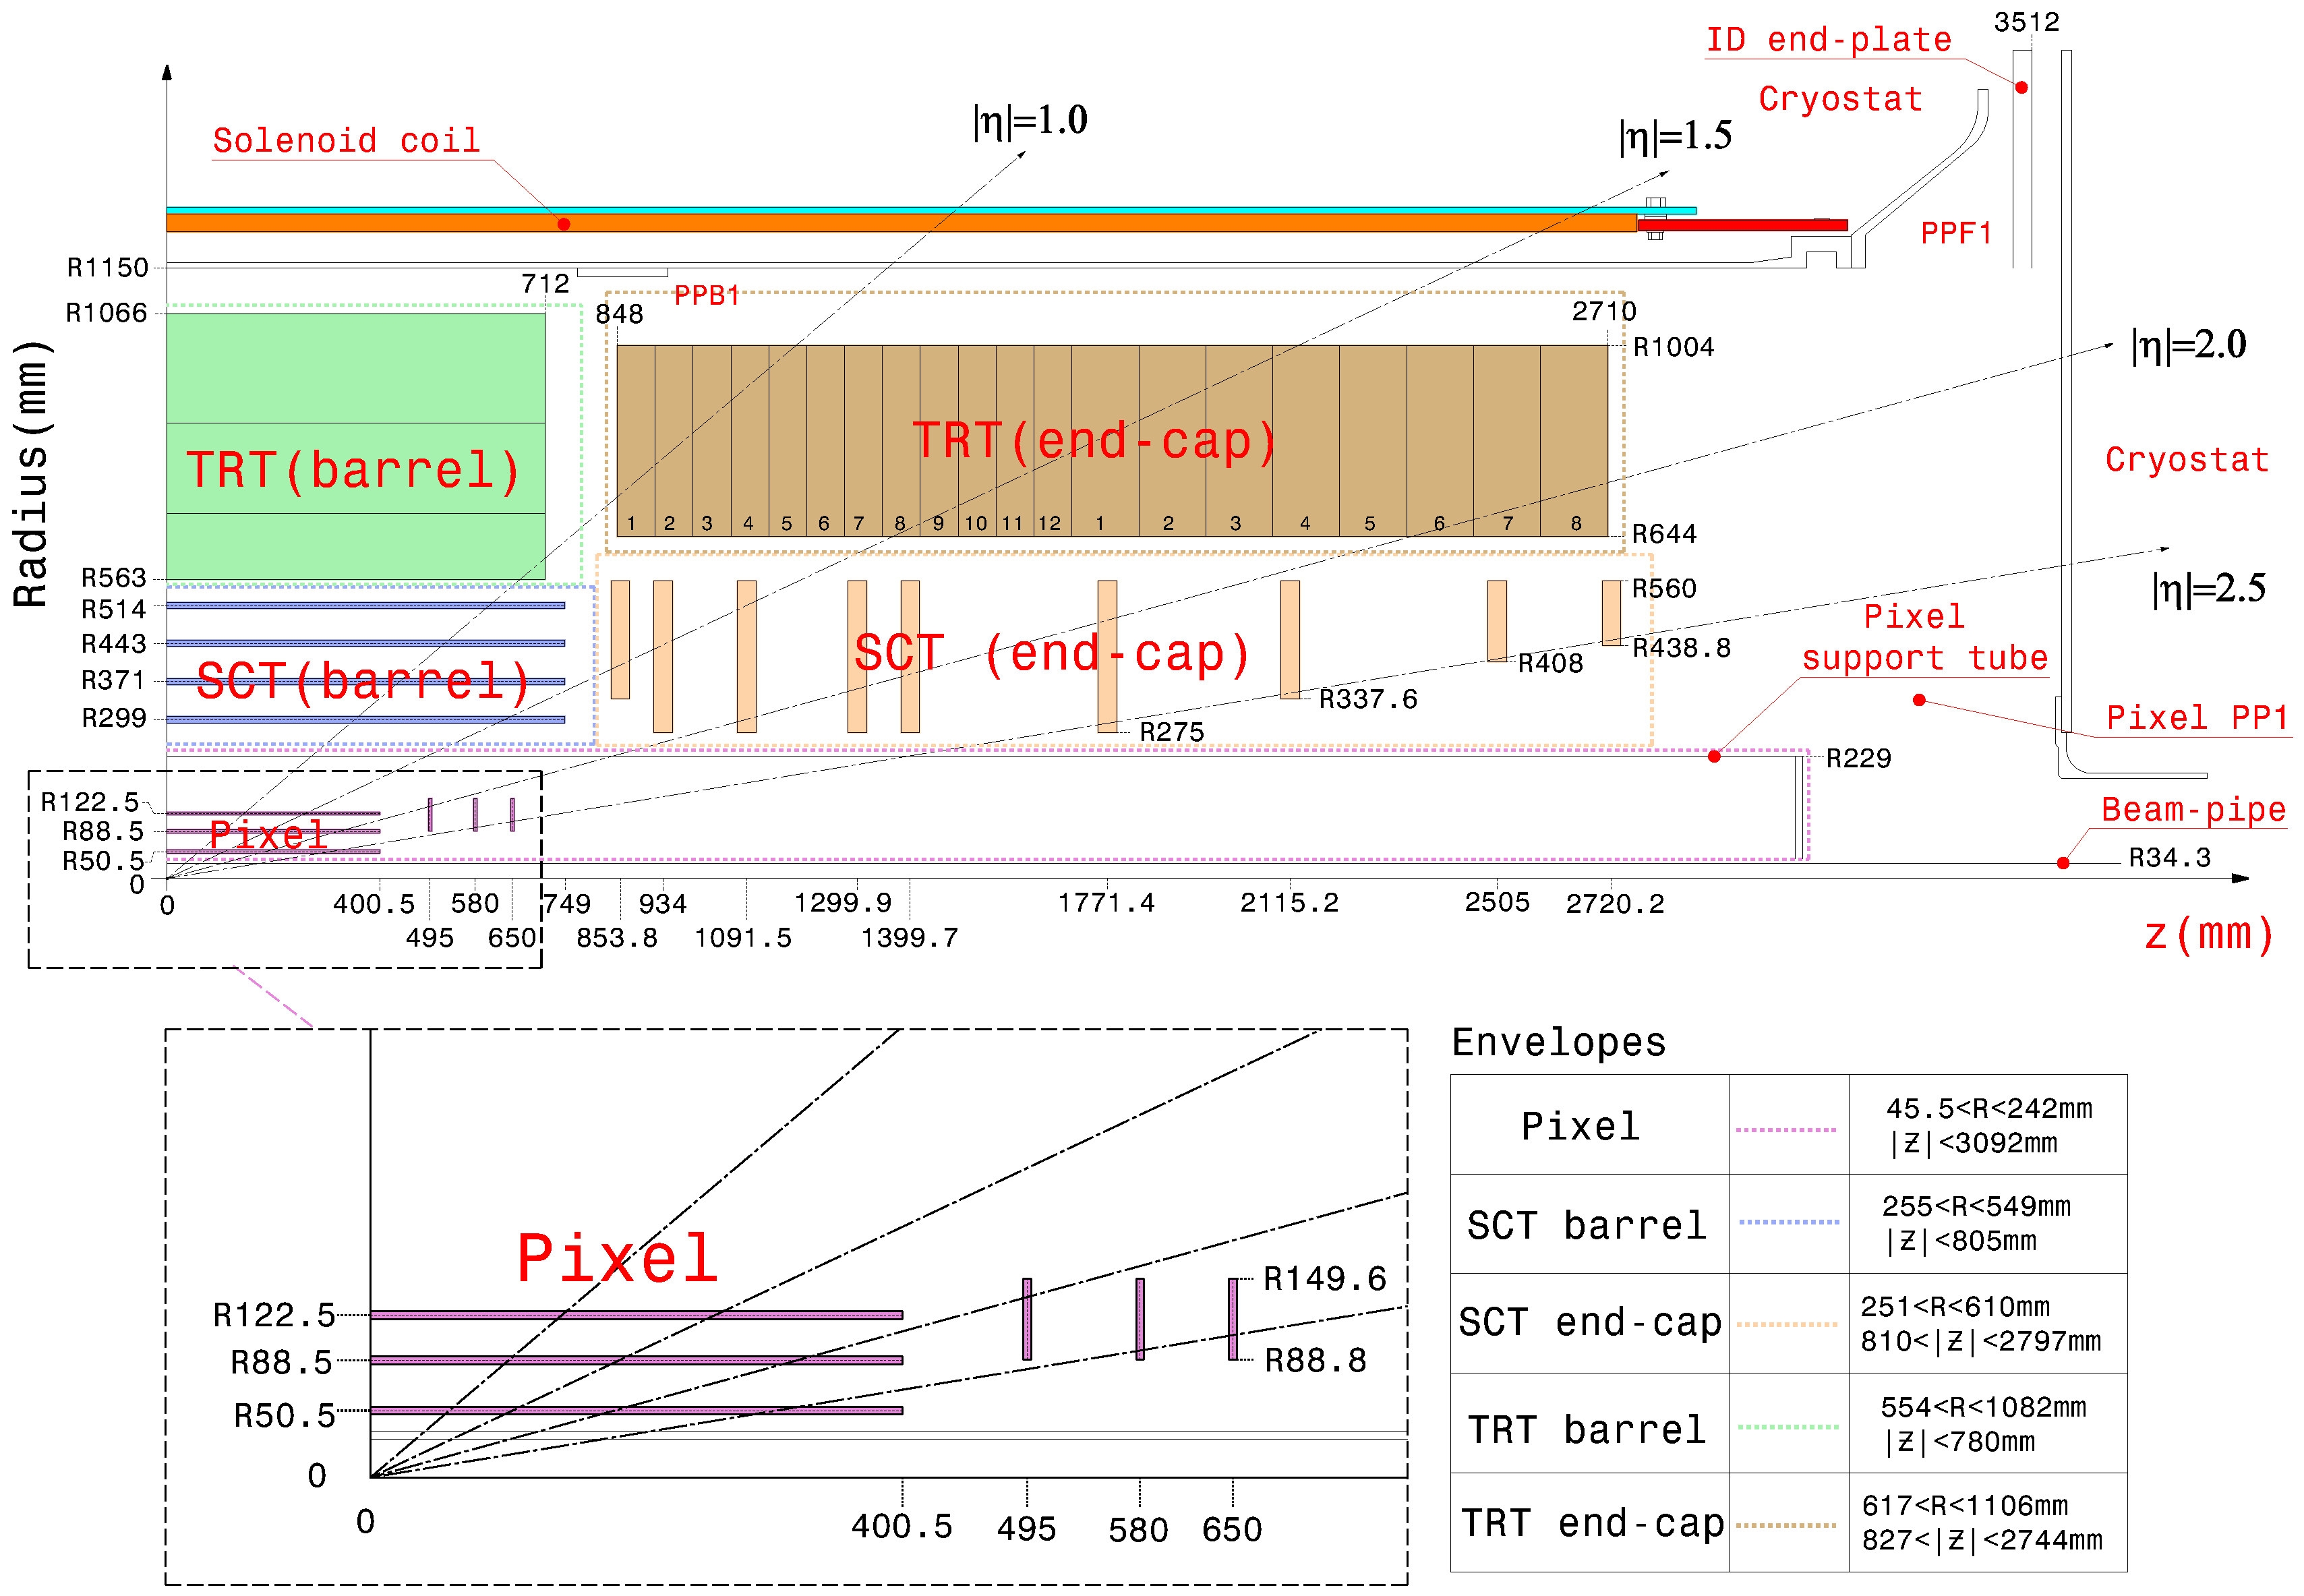
\includegraphics[width=0.45\textwidth, angle=0]{figures/LHC_ATLAS/FigID26-mod-011107.eps}
\caption{ (a) Cutaway view of the ATLAS inner detector. (b) Radial View of the ATLAS inner detector (Figure Taken from \cite{ATLAS_JINST}) \label{LHC:fig:ATLASID}}
%\end{center}
\end{figure}

\indent More detail on each sub-detector technology is given below. \\

\subsubsection*{ Pixel Detector and the Insertable B-Layer}

\indent The Pixel detector consists of three layers of high resolution pixel sensors in the cylindrical barrel and three wheels of pixel sensors in the endcap.  Another inner most layer of pixel sensors called the Insertable B-Layer (IBL) was added directly on top of the new beryllium beam pipe in the first long shutdown between 2012 and 2015.  The new beam pipe decreases the amount of multiple scattering before the inner tracker. \\

\indent The original 3 layer Pixel detector contain of 80.4 million readout channels spread over 1744 Pixel modules.  Each module house a sensor tile with an area of $63.4 \times 25.4$ mm$^2$.  The sensors are composed of 250 $\mu$m thick n-type silicon wafer pixels with a size of $50\times400 \mu$m$^2$. The modules are read out by 16 front-end electronic chips with 2880 read out channel each. \\

\indent The pixels have an intrinsic accuracy of 10 $\mu$m in the bending $\phi$ direction and 115 $\mu$m accuracy in the non-bending $z$ direction in the barrel and $\phi$ direction in the endcap.\\ 

\indent Installed in 2014, the Insertable B-Layer (IBL) contributes another 12 million channels to the Pixel system in Run 2.\cite{IBLOverview,IBL_TDR}  Located directly on top of the beam pipe at 3.3 cm from the beam axis, the IBL is the new most inner layer of the Pixel detector ( the previous innermost B-Layer was at 5 cm). The IBL is composed of 14 staves tilted at $14^{\circ}$ in $\phi$.  A schematic representation of IBL stave relative to the beam pipe can be seen in figure \ref{LHC:fig:IBL}Each stave is equipped with 32 FE-I4 front-end chip bonded to silicon sensors. Each FE-I4 chip contain 26880 pixel cells with $50 \times 240$ $\mu$m pitch.\\

\indent The improvement in both the tracking lever arm and spacial resolution represent approximately a factor of 2 impact parameter resolution and a factor of 4 gain in b-tagging light jet rejection power. \\

\begin{figure}[h!]
%\begin{center}
\centering
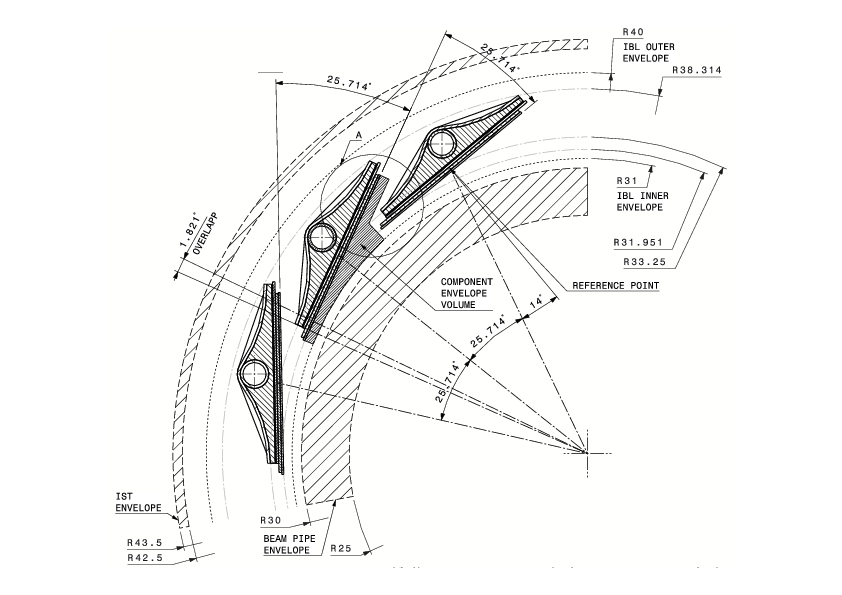
\includegraphics[width=0.55\textwidth, angle=0]{figures/LHC_ATLAS/fig_ibl_layout_rev.png}
\caption{ Schematic of the ATLAS Insertable B-Layer (IBL) (Figure Taken from \cite{IBLOverview}) \label{LHC:fig:IBL}}
%\end{center}
\end{figure}

\subsubsection*{ Semiconductor Tracker}

\indent The SCT is composed of 4 coaxial layers of concentric cylinders in the barrel and 9 disks in each endcap and contributes at least an additional 4 layers of high precision position measurements to tracks originating from the IP in the intermediate radial range.  The entire SCT consists of approximately 6.3 million readout channels on over 4088 modules.  A barrel module is equiped with a sensor with a size of $64.0 \times 63.6$ mm$^2$ in the transverse plane.  The barrel sensor are made of 285 $\mu$m thick silicon wafer and contain 768 strips, achieving a barrel strip-pitch of 80 $\mu$m.  The endcap module contain sensors that are trapezoidal in shape with strip pitch that vary from 54 $\mu$m to 90 $\mu$m.  \\

\indent The sensors are mounted on a back to back fashion at angle of $40$ mrad relative to one another.  This allows the measurement of non-bending direction along with improved spacial resolution in the bending $\phi$ direction.  \\

\indent   The intrinsic accuracy per SCT module, dictated by the strip pitch, is 17 $\mu$m in the bending $\phi$ direction and 580 $\mu$m in the non-bending z direction in the barrel and R direction in the endcap.\\

\subsubsection*{Transition Radiation Tracker}

\indent The TRT is the outermost component of the ID and contribute approximately 351000 readout channels.  Each channel correspond to a 4 mm diameter polyimide straw drift tube with a $31 \mu$m gold plated tungsten anode wire, providing an intrinsic accuracy of 130 $\mu$m.  The number of channels is low compared to the silicon detectors but the TRT is able to compensate for this by providing a long lever arm to the track measurement and high hit multiplicity.  \\

\indent In the barrel region, the straws are 144 cm long and arranged parallel to the beam axis in 73 layers . In the end-cap region, straws are 37 cm long and arranged in 160 radial layers in wheels.  A typical track will traverse 36 straws in the barrel, because the tubes are arranged a matrix with each layer offset from one another.\\

\indent The dielectric material used to interleave the straws induces transition radiation in traversing charged particles.  The low energy transition radiation photons are absorbed by the Xenon-based gas mixture in the straws, thereby providing much larger signal amplitudes than minimum-ionizing charged particles.  This can be used to distinguish electrons from pions based on the energy deposition.  \\

\indent In 2015 and 2016 operations, approximately $1/3$ to $2/3$ of the TRT barrel and $1/7$ of the TRT endcap is filled with an Argon gas mixture instead of Xenon due to leaks.  This adversely affects electron identification efficiency by a few percent and is taken into account by a scale factor electron identification in simulation.  \\

\subsection{The Calorimeter}
\label{LHC:Calorimeter}

\indent The ATLAS calorimeter provide near full solid angle coverage of the interaction point up to an $\eta$ of 4.9.  The calorimeter system is composed of two parts the electromagnetic calorimeter (ECAL) and hadronic calorimeter (HCAL).  These two detector technology use scintillating tiles and liquid argon (LAr) as active materials.  The design resolution for electromagnetic objects is $\sigma_E/E = 10\%/\sqrt{E} \oplus 0.2\%$.  Measurements from pions give a hadronic energy resolution of $\sigma_E/E = (56.4\pm0.4)/\sqrt{E}\oplus(5.4\pm0.1)$ in the barrel region to $\sigma_E/E = (94.2\pm1.6)/\sqrt{E}\oplus(7.5\pm0.4)$ in the forward regions. \\

\indent The cutaway view of the ATLAS calorimeter can be seen in figure \ref{LHC:fig:ATLASCalo} and a summary of the calorimeter geometry is given in table \ref{} \\

\begin{figure}[h!]
%\begin{center}
\centering
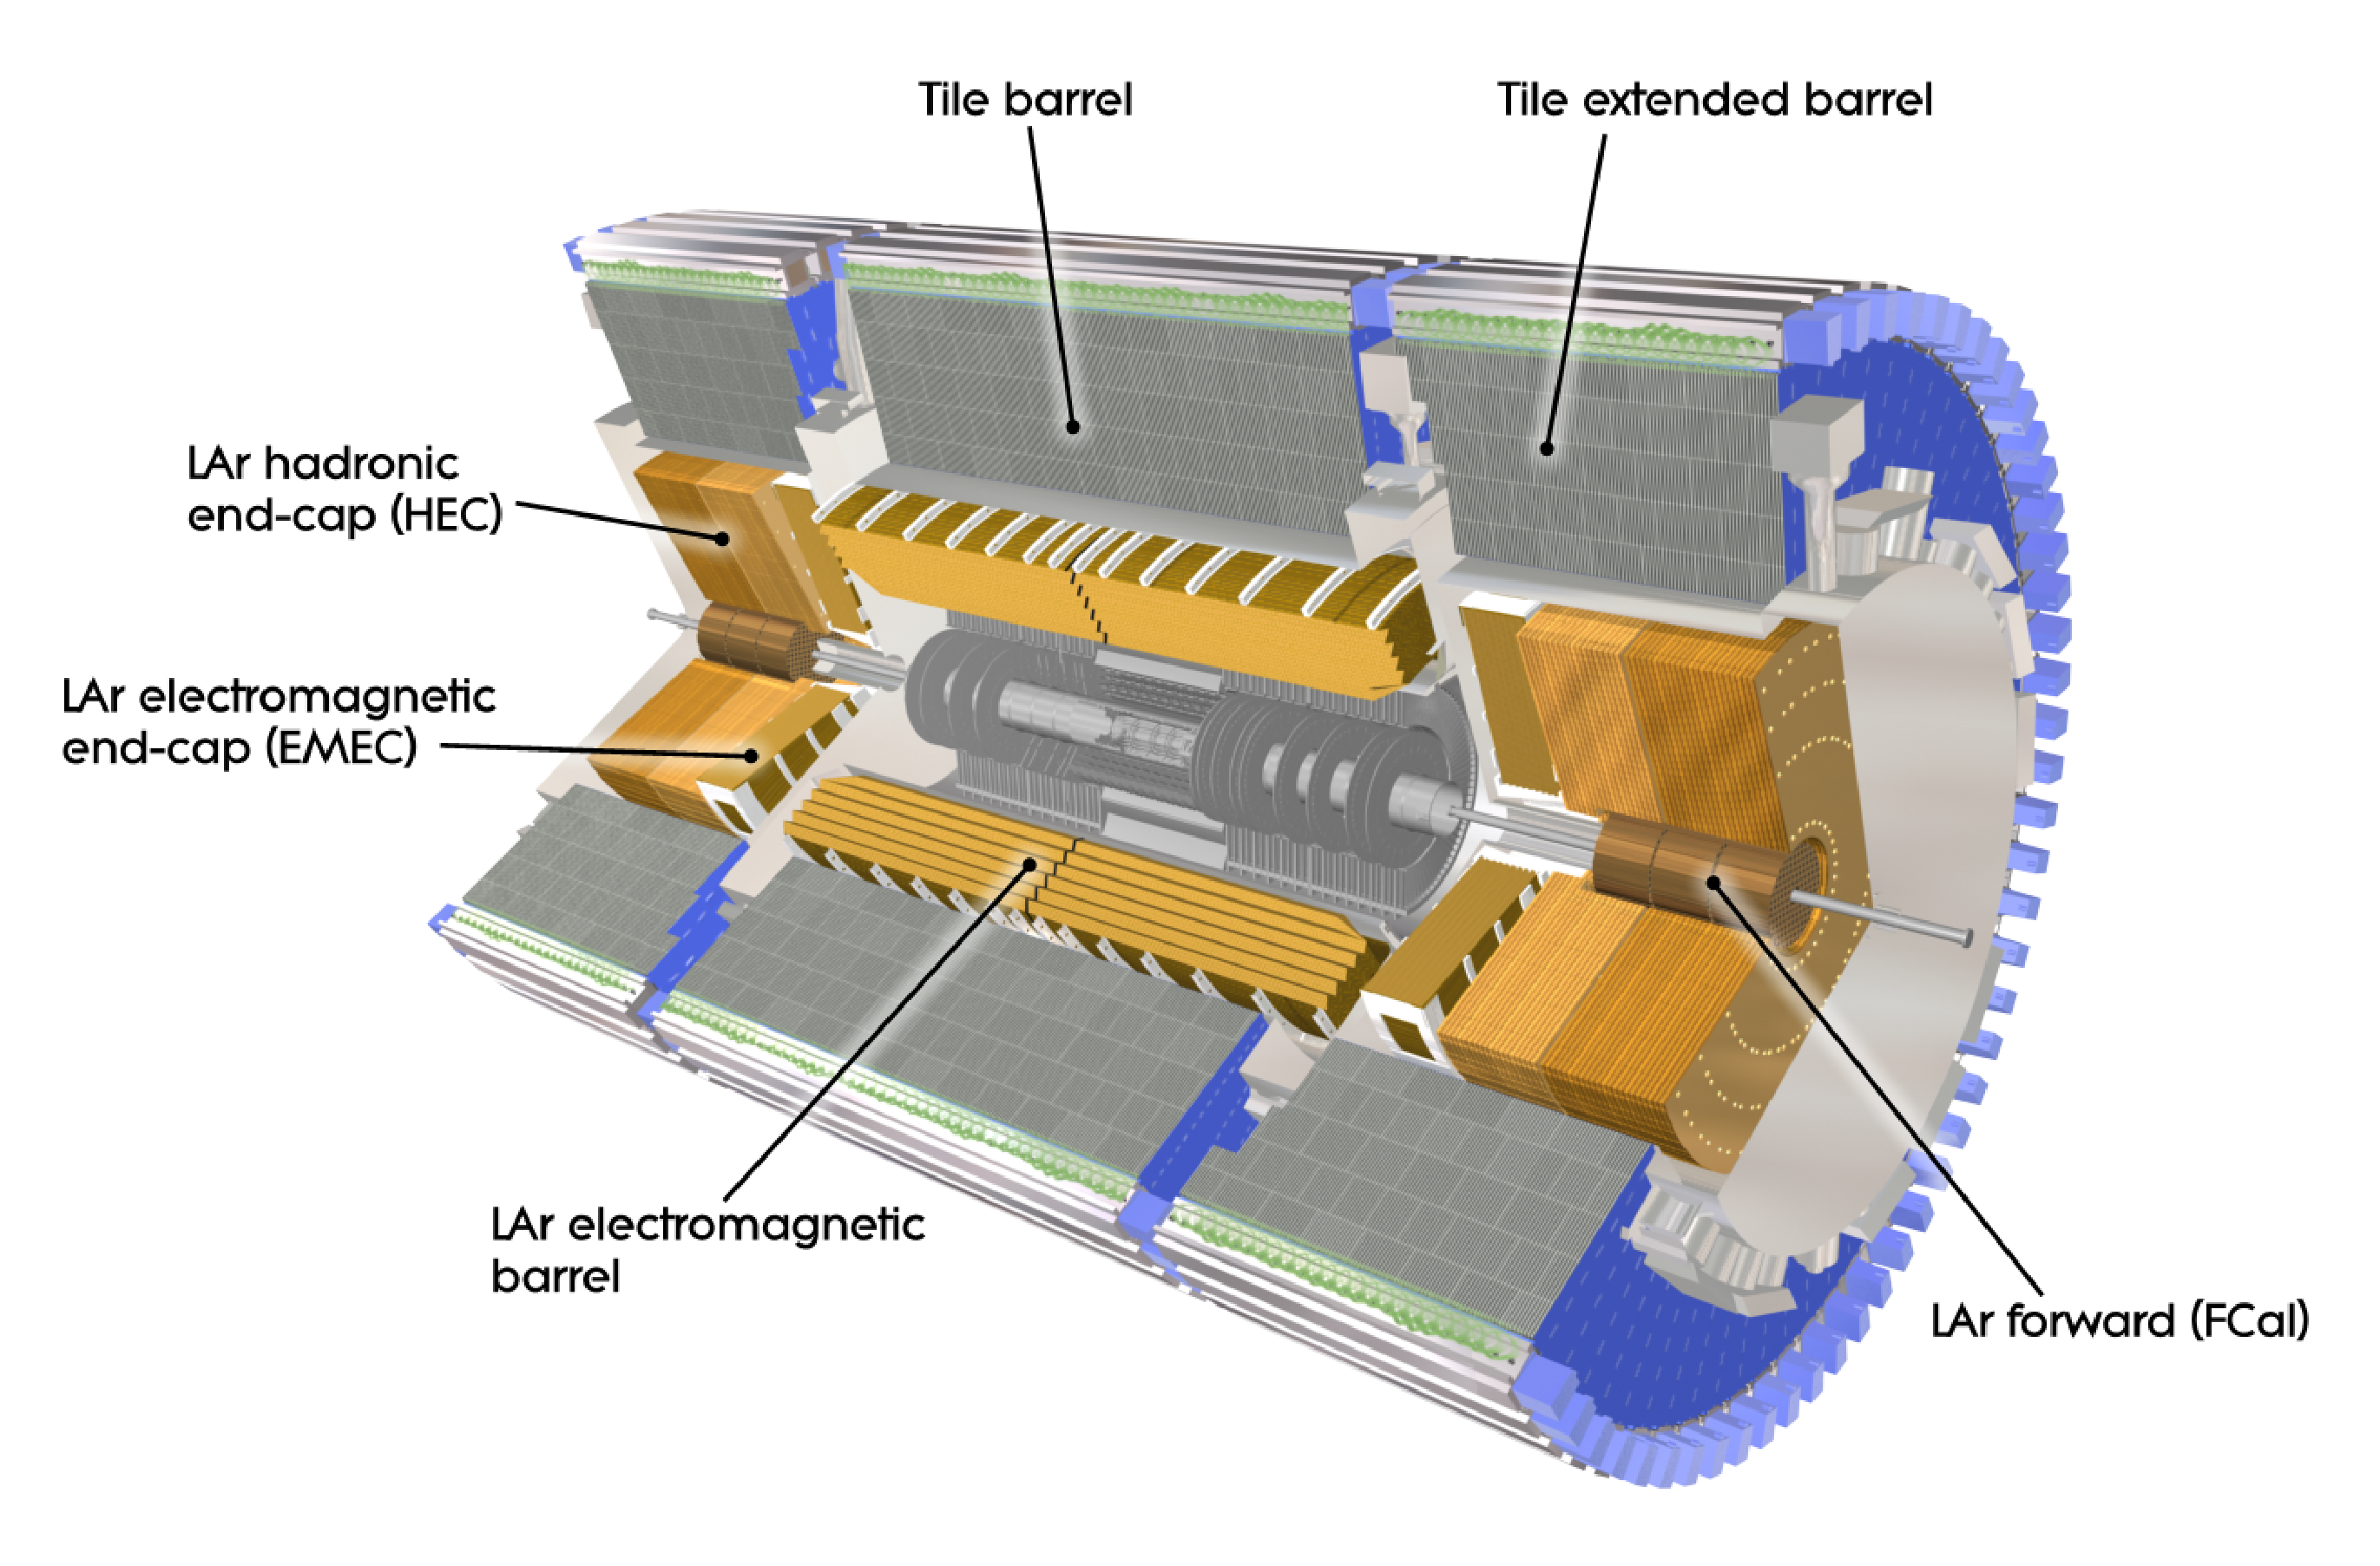
\includegraphics[width=0.75\textwidth, angle=0]{figures/LHC_ATLAS/Calorimeter_d3.eps}
\caption{ Layout of the ATLAS calorimeter. (Figure taken from \cite{ATLAS_JINST}) \label{LHC:fig:ATLASCalo}}
%\end{center}
\end{figure}

\subsubsection*{Electromagnetic Calorimeter}

\indent The ATLAS ECAL is sampling calorimeter with lead absorber plates and liquid argon (LAr) active material arranged in an accordion geometry covering up to an $\eta$ of $3.2$.  The accordion design provides full crack-less coverage in $\phi$ and integrates more charge along the longitudinal direction of the shower.  \\

\indent The ECAL is split into a barrel and two endcap components with a transition region of $1.37 < |\eta| < 1.52$ in between.  The barrel component is divided into two 3.2 m long half-barrel sections with an inner and outer radius of 2.8 m and 4 m respectively.  The endcap is divided into two coaxial wheels each 63 cm thick with an outer wheel covering $1.375 < |\eta| < 2.5$, and an inner wheel covering the region $2.5 < |h| < 3.2$. \\

\indent The barrel ECAL is also segmented longitudinally into 3 layers with an additional presampler layer in front in certain regions.  The presampler is from from a thin liquid-argon layer 11mm in depth and is designed to determine the energy loss from material upstream of the calorimeter.  The first layer after the presampler has a depth of 4.3 radiation length ($\Chi_0$) and a fine granularity of $\Delta\eta \times \Delta\phi = 0.003 \times 0.1$.  The high granularity allows for precision measurement of EM showers and can distinguish between the shower shape of electron/photons from those of $\pi^0\rightarrow \gamma\gamma$ decays.  The middle layer absorbs most of the energy of the EM shower and are made up of cells with $\Delta\eta \times \Delta\phi = 0.025 \times 0.025$ with a depth of $16 \Chi_0$.  The back layer has cell sizes of $\Delta\eta \times \Delta\phi = 0.05 \times 0.025$ a depth of $2 \Chi_0$.  The back layer is designed to only collect the tails of the EM showers and used to distinguish between EM and hadronic showers.  \\

\indent The endcap ECAL is also divided into three longitudinal layers similar to the barrel.  The front layer has a depth of 4.4 $\Chi_0$ and varies in cell size from $\Delta\eta \times \Delta\phi = 0.003 \times 0.1$ to $\Delta\eta \times \Delta\phi = 0.006 \times 0.1$. The middle layer has cells with the same size as the barrel with $\Delta\eta \times \Delta\phi = 0.025 \times 0.025$. and a similar depth. The back layer has a twice coarser granularity in $\eta$ with $\Delta\eta \times \Delta\phi = 0.05 \times 0.25$.  A presampler also exists for the endcap with each presampler module consisting of two 2mm thick LAr layers. \\

\indent The segmentation of the ATLAS ECAL can be seen in figure \ref{LHC:fig:EMCalo}. \\

\begin{figure}[h!]
%\begin{center}
\centering
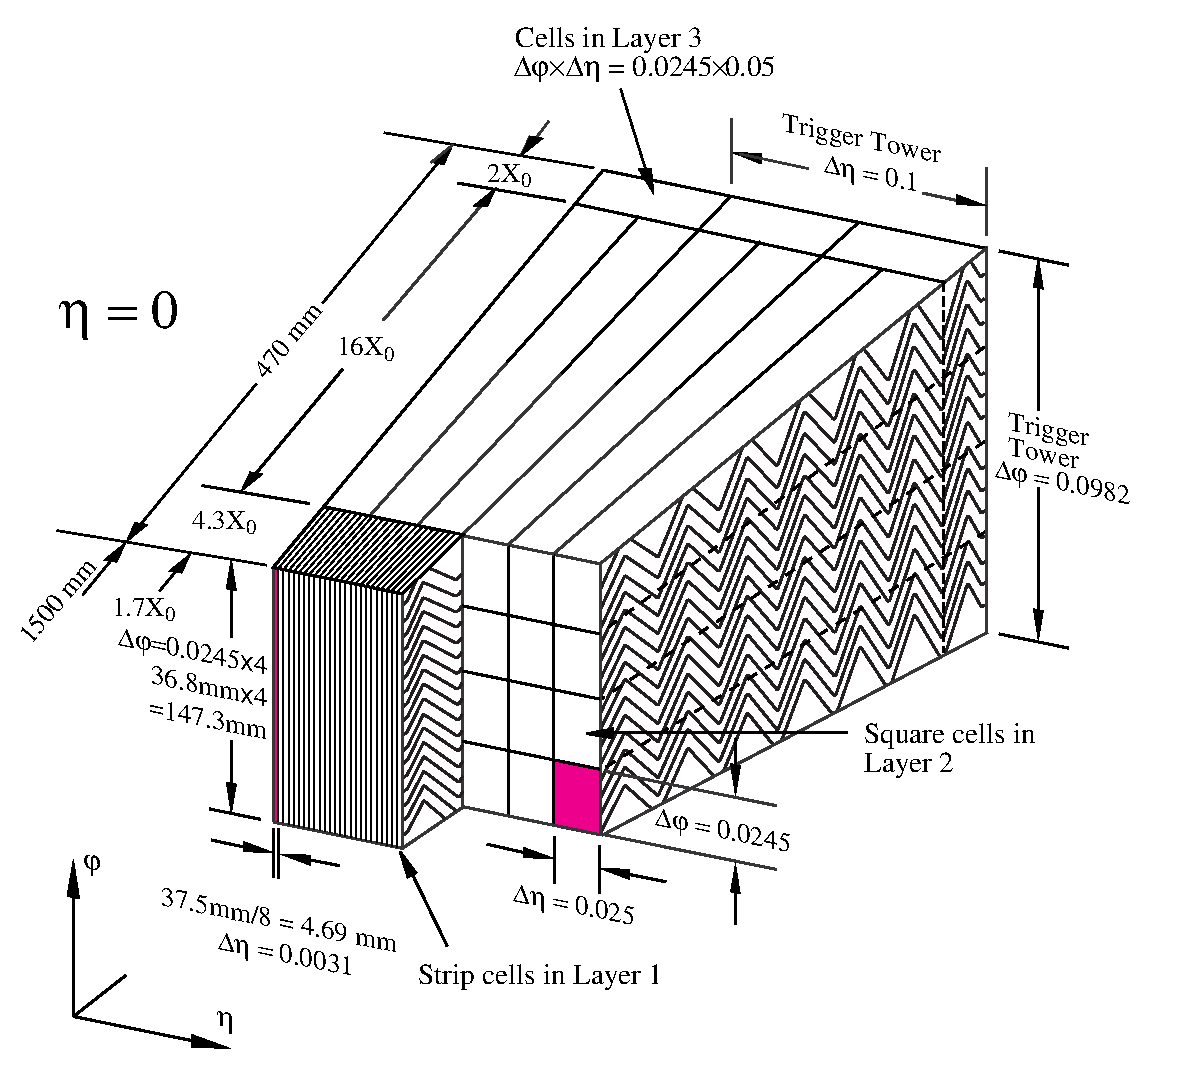
\includegraphics[width=0.40\textwidth, angle=0]{figures/LHC_ATLAS/LARG3-TDR-barrelM.eps}
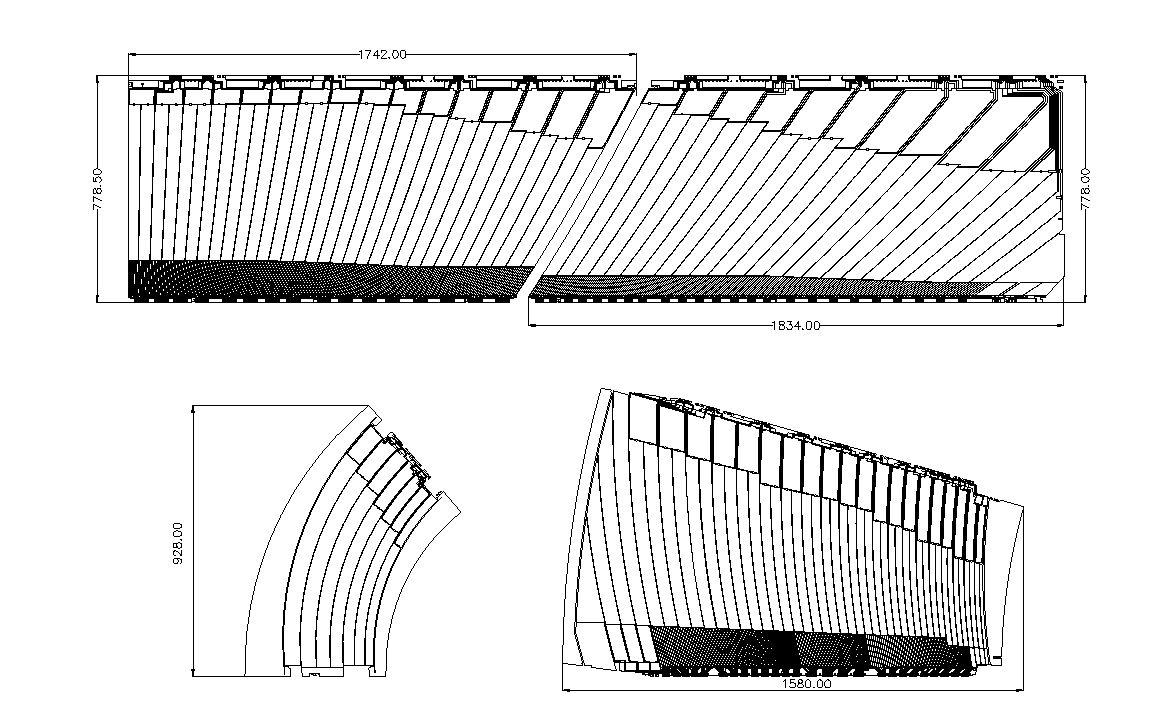
\includegraphics[width=0.50\textwidth, angle=0]{figures/LHC_ATLAS/LARG3-abcdM.eps}
\caption{ (a) The three layers of the EM module with the accordion geometry show. (b) Orientation of EM cells in the barrel and endcap relative to the IP.  Cells are orientated to point back to the IP.  (Figures taken from \cite{ATLAS_JINST}) \label{LHC:fig:EMCalo}}
%\end{center}
\end{figure}

\indent The total thickness of the ECAL is at least $22 \Chi_0$ in the barrel and $24 \Chi_0$ in the endcap for electrons and photons and approximately 1.5 nuclear interaction length for hadronic objects. \\

\subsubsection*{Hadronic Calorimeter}

\indent The ATLAS HCAL is directly outside the ECAL and is responsible for containing and measuring the energy of hadronic showers.  The HCAL consists of 3 separate detectors covering different $\eta$ regions, the tile calorimeter, the LAr endcap calorimeter (HEC) and the LAr forward calorimeter (FCal).  \\

\indent The tile calorimeter is a sampling calorimeter using steel absorbers and scintillating tiles as active material. The barrel tile calorimeter covers an $\eta$ range of $|\eta| < 1.0$ and two extended barrel tile calorimeter covers the $0.8 < |\eta| < 1.7$ region.  Both barrel and extend barrel calorimeters are divided in $\phi$ into 64 modules each with $\Delta\phi = 0.1$.  Each module is segmented in the radial direction with 3 layers.  The 3 layers have an approximate thickness of 1.5, 4.1 and 1.8 nuclear interaction lengths ($\lambda$) in the barrel and 1.5, 2.6, and 3.3 $\lambda$ in the extended barrel.  Two sides of the scintillating tiles are read out by two separate photomultiplier tubes. \\

\indent A Schematic view of a tile calorimeter module can be seen in figure \ref{LHC:fig:TileCalo}

\begin{figure}[h!]
%\begin{center}
\centering
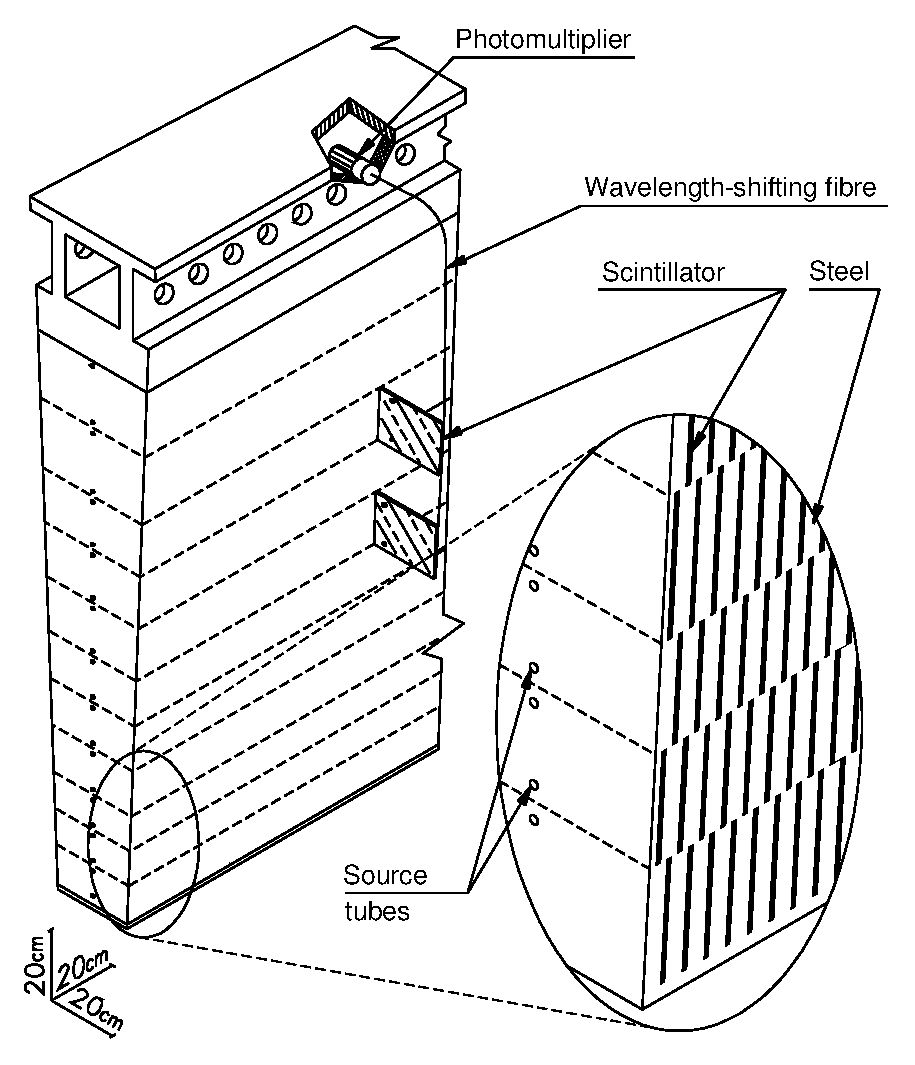
\includegraphics[width=0.45\textwidth, angle=0]{figures/LHC_ATLAS/TileCal_Module3.eps}
\caption{ The tile calorimeter module with steel absorber, tile scintillators and photomultiplier readout.  (Figures taken from \cite{ATLAS_JINST}) \label{LHC:fig:TileCalo}}
%\end{center}
\end{figure}


\indent The HEC uses LAr as the active material and copper as the absorber material with copper plates interleaved with LAr gaps.  The HEC is located directly behind the ECAL endcap and share the ECAL cryostat.  Covering an $\eta$ range of $1.5<|\eta| < 3.2$ the HEC overlaps slightly with the tile calorimeter and FCAL in order to minimize a drop in material density.  Geometrically the HEC consists of two independent wheels per endcap with each wheel segmented in $\phi$ into 32 wedge shaped modules.  Each HEC module is composed of cells with a size of $\Delta\eta \times \Delta\phi = 0.1 \times 0.1$ for the $|\eta|<2.5$ region and $\Delta\eta \times \Delta\phi = 0.2 \times 0.2$ in higher eta regions.  The HEC model is also segmented longitudinally into two sections making a total of 4 layers. The combined depth of all 4 layers is approximately 10 interaction lengths. \\

\indent The FCal is an LAr sampling calorimeter that extends the $\eta$ coverage of the HCAL to 4.9.  A compact design with very small LAr gaps was chosen for this high flux region.  The FCal is segmented in the longitudinal direction with 3 distinct modules. The absorber material is copper for the first module and tungsten in the last two.  The copper absorber is optimized for EM measurements while the tungsten is predominantly designed for hadronic interactions.  The 3 modules combined achieves a depth of 10 nuclear interaction length. \\

\subsection{The Muon Spectrometer}
\label{LHC:MuonSpec}

\indent The muon spectrometer consist of three layers of precision tracking chambers to track the path of muons in the bending $\eta$ direction.  The precision tracking chambers is composed mainly of the Monitored Drift Tube (MDT) detector with the Cathode Strip Chamber (CSC) detector used in the forward region.  Alongside the precision trackers are fast trigger chambers, the Resistive Plate Chambers (RPC) in the barrel and the Thin Gap Chambers (TGC) in the endcap. \\

\indent The configuration of the muon system is shown in figure \ref{LHC:fig:ATLASMuonSpec} ~\\

\begin{figure}[h!]
%\begin{center}
\centering
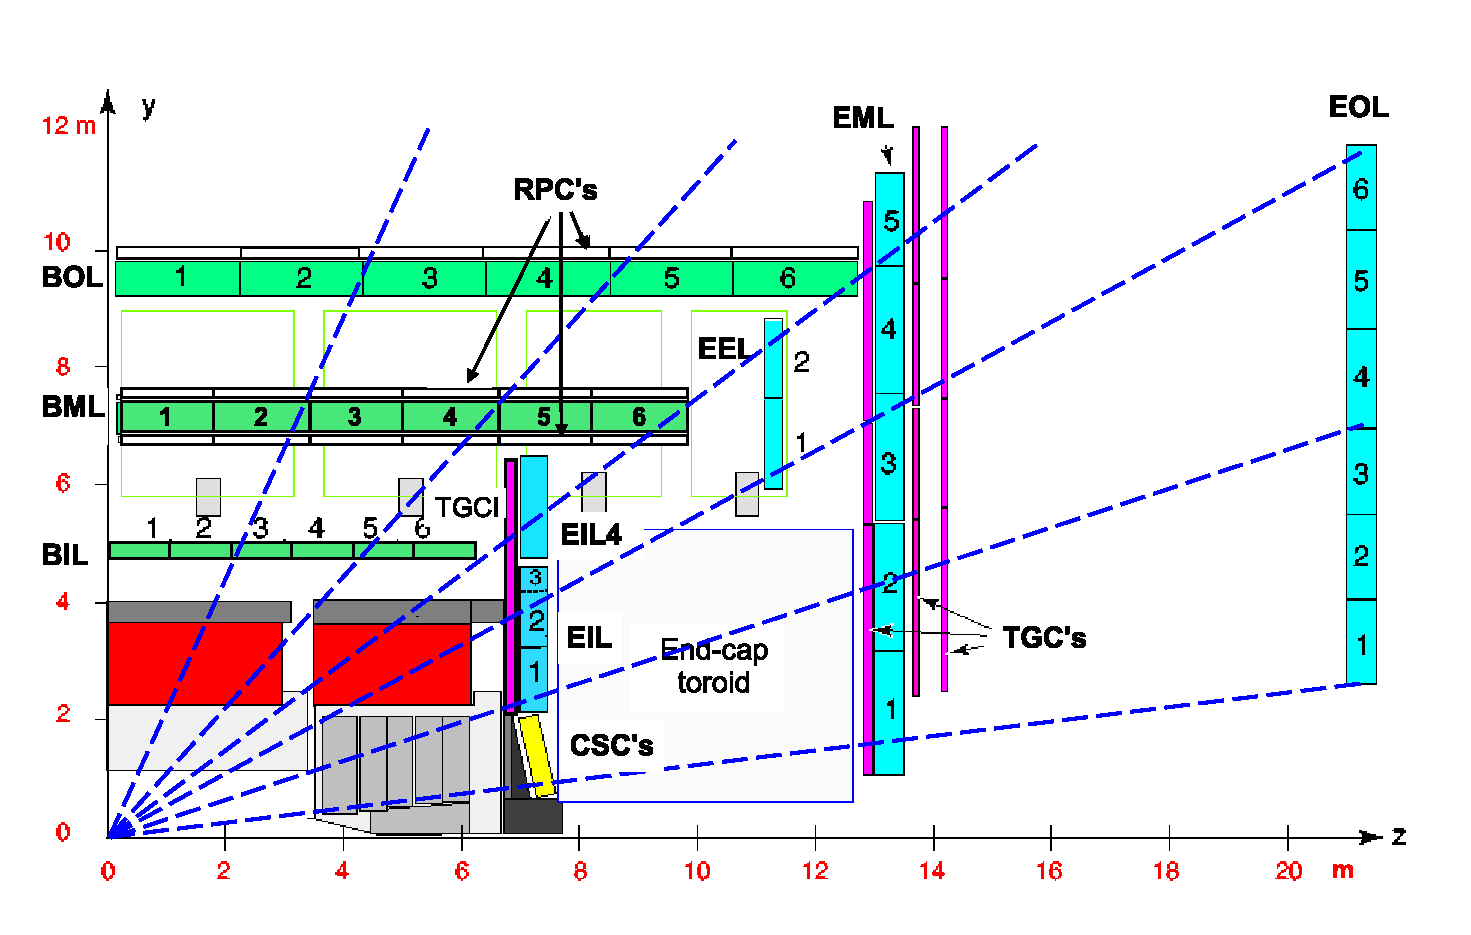
\includegraphics[width=0.75\textwidth, angle=0]{figures/LHC_ATLAS/Muon_rz_large_sect_6.eps}
\caption{ Cutaway view of the ATLAS Muon Spectrometer.  (Figure taken from \cite{ATLAS_JINST}) \label{LHC:fig:ATLASMuonSpec}}
%\end{center}
\end{figure}

\indent Eight air core superconducting toroid magnets in the barrel and eight superconducting toroid magnets in the endcaps provide 1.0 Tm to 7.5 Tm of bending power in the MS volume. The barrel magnets cover an |$\eta$| range of 1.4 and the endcap magnets cover an |$\eta$| range from 1.6 to 2.7. The area between $1.4 < |\eta| < 1.6$ is called the transition region and has a mixed magnetic field from both the barrel and endcap. The endcap magnets are offset from the barrel magnets by 22.5 degrees in the $\phi$ direction to allow a smoother magnetic field in this region. The configuration of the magnets is shown in figure \ref{LHC:fig:ATLASMag} ~\\

\begin{figure}[h!]
%\begin{center}
\centering
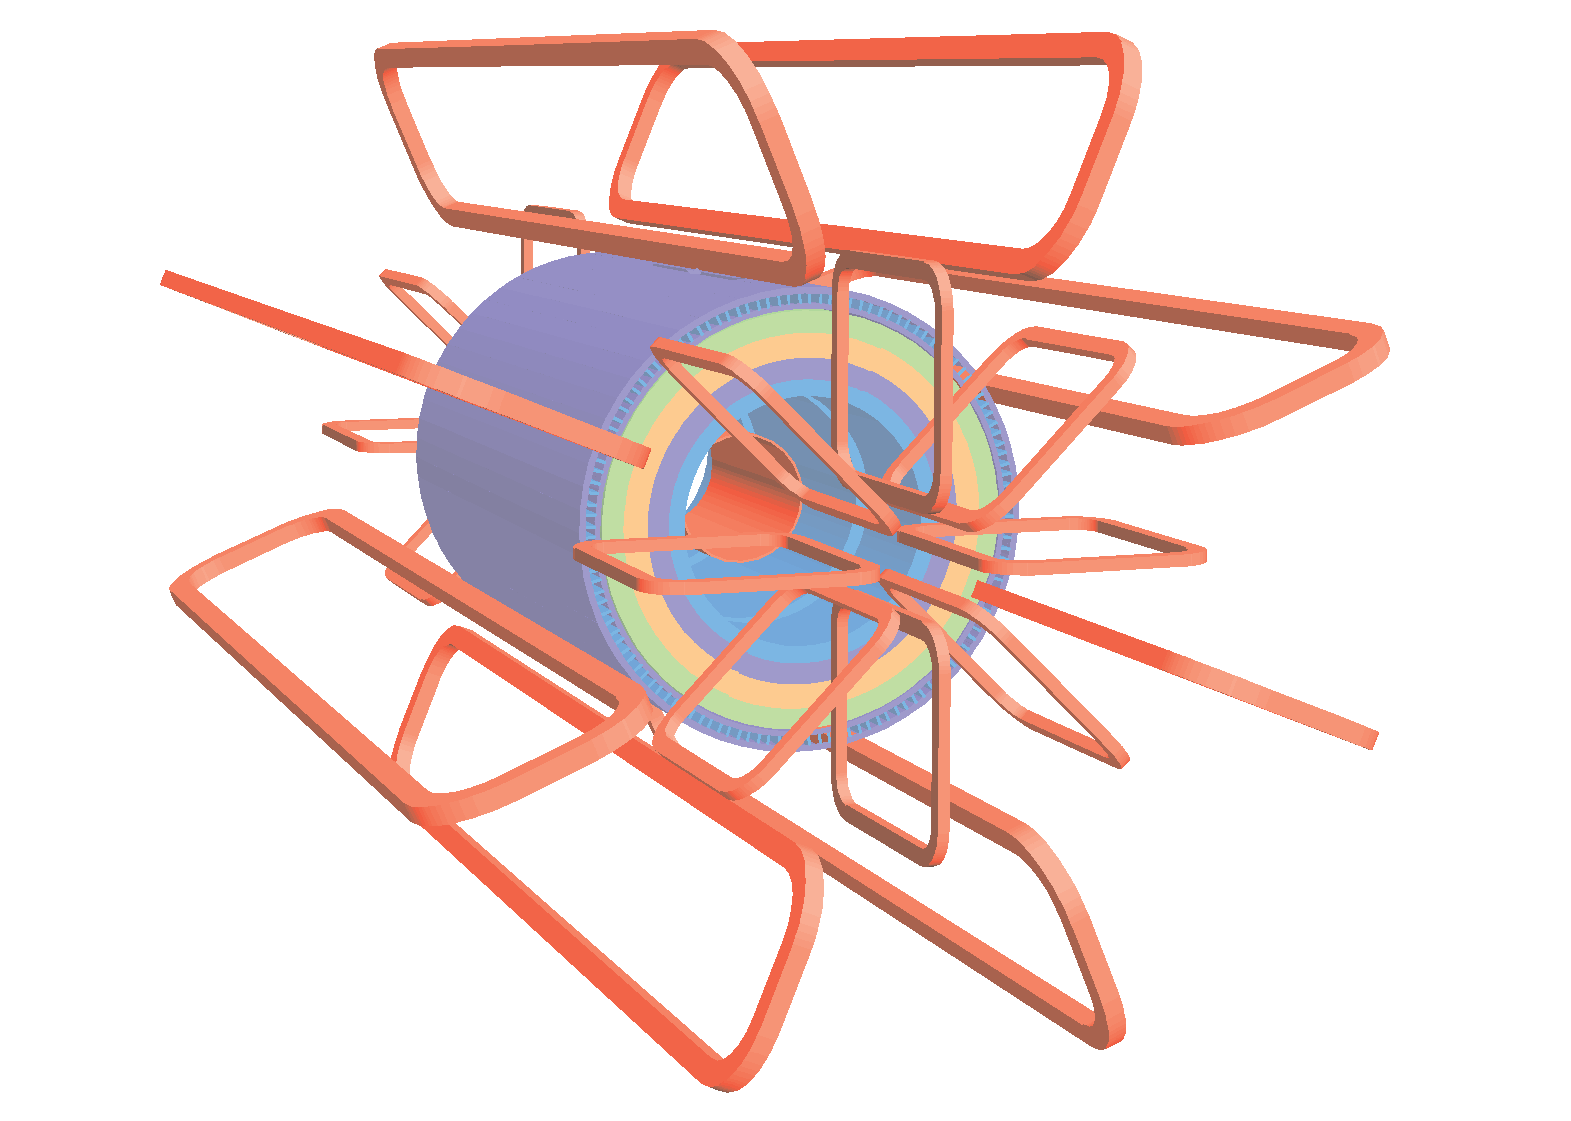
\includegraphics[width=0.60\textwidth, angle=270]{figures/LHC_ATLAS/ATLcoilGeom.eps}
\caption{ Geometry of the barrel and endcap toroid magnets. The cylinder repesents the calorimeter. (Figure taken from \cite{ATLAS_JINST}) \label{LHC:fig:ATLASMag}}
%\end{center}
\end{figure}

\indent The MS is designed to be able to detect muon candidates with a wide range of momenta from $3 \gev to 3 \tev$ with standalone muon momentum resolution of $\sigma_{\pt}/\pt = 10\%$ at a $\pt$ of 1 TeV.  The open design of the MS minimizes multiple scattering after the calorimeter and gives a large lever arm for high momentum resolution. \\

\subsubsection*{Muon Precision Tracking}

\indent The ATLAS MS system consist of 3 stations of muon precision tracking chambers at approximately 5 m, 7.5 m and 10 m radii in the barrel and 7.4 m,14 m and 21.5 m in $z$ the endcap covering an $|\eta| < 2.7$.  Each chamber consists of 3 to 8 layers of MDT tubes.  The only exception to this is the very high rate region in the inner endcap at high $\eta$ which uses CSC technology.\\

\indent  MDT tubes are 3cm diameter aluminum tubes filled with Ar/CO$_2$ gas mixture with a tungsten-rhenium anode wire.  Each tube have an intrinsic resolution of 80 $\mu$m corresponding to a resolution of $35 \mu$m per chamber and offer measurements in the bending $\eta$ direction.  \\

\indent CSC are multiwire proportional chambers with one layer of anode wires in the bending plane and two layers of cathode strips. The position of the track is obtained by interpolation between the signal on neighboring cathode strips. The CSC wire signals are not read out. The strips are perpendicular to one another with 5.31mm (5.56mm) pitch in the bending plane and 12.5 mm (21.0 mm) for small (large) chambers.  This offers an $60 \mu$m resolution per plane in the bending plane and about 5 mm resolution in the non-bending plane. \\

\indent The structure of MDT tubes and CSC chambers can be seen in figure \ref{LHC:fig:MDT} and \ref{LHC:fig:MDT} . \\

\begin{figure}[h!]
%\begin{center}
\centering
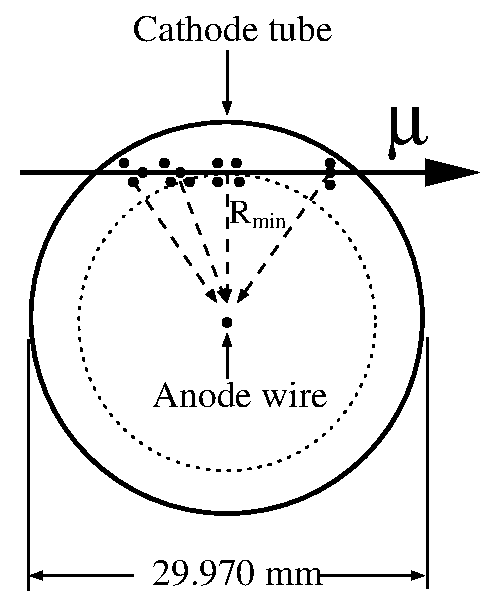
\includegraphics[width=0.30\textwidth, angle=0]{figures/LHC_ATLAS/MDT_tube_cross_section.eps}
\caption{ Schematic Representation of MDT tubes (Figures taken from \cite{ATLAS_JINST}) \label{LHC:fig:MDT}}
%\end{center}
\end{figure}

\begin{figure}[h!]
%\begin{center}
\centering
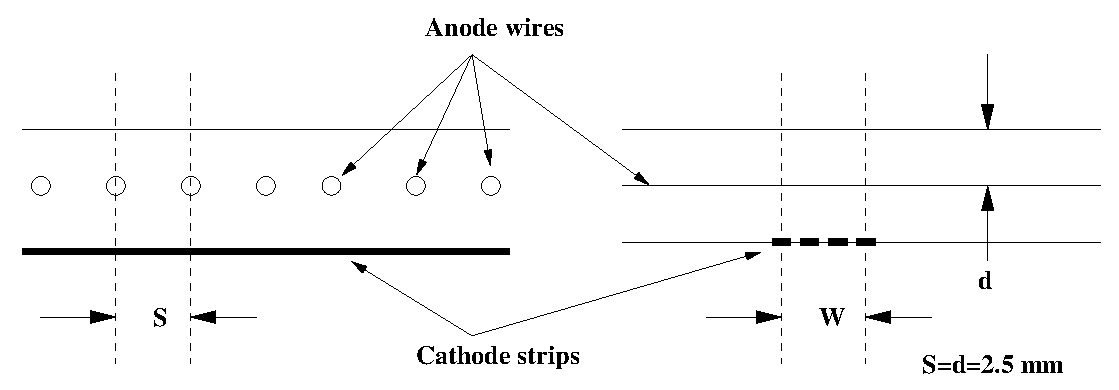
\includegraphics[width=0.85\textwidth, angle=0]{figures/LHC_ATLAS/CSC_structure.eps}
\caption{ Schematic Representation of CSC chambers. (Figures taken from \cite{ATLAS_JINST}) \label{LHC:fig:MDT}}
%\end{center}
\end{figure}

\subsubsection*{Muon Trigger Chambers}

\indent  The ATLAS MS also features a system of fast trigger chambers consisting of three station of Resistive Plate Chambers (RPC) in the barrel and 4 stations of Thin Gap Chambers (TGC) in the endcap.  The MS triggering system provide triggering up to an $\eta$ of 2.4.  The RPCs are placed below and above the middle MDT station and outside the outer MDT barrel station.  The TGC stations are arranged with one station in front of the inner endcap precision tracking wheel and 3 stations split in front and behind the middle endcap MDT wheel.  The trigger searches for fast coincidences between the layers along the expected trajectory of a muon.  Different maximum deviation from the straight path is allowed for triggers with different thresholds momenta. \\

\indent In Run 2, muon triggers in the endcap also require coincidences in the inner layer of the TGC to reduce rates of fake triggers due to particles interacting with beam shielding in the forward region. \\

\indent A schematic of the muon trigger system is given in figure \ref{LHC:fig:MS_trigger}. \\

\begin{figure}[h!]
%\begin{center}
\centering
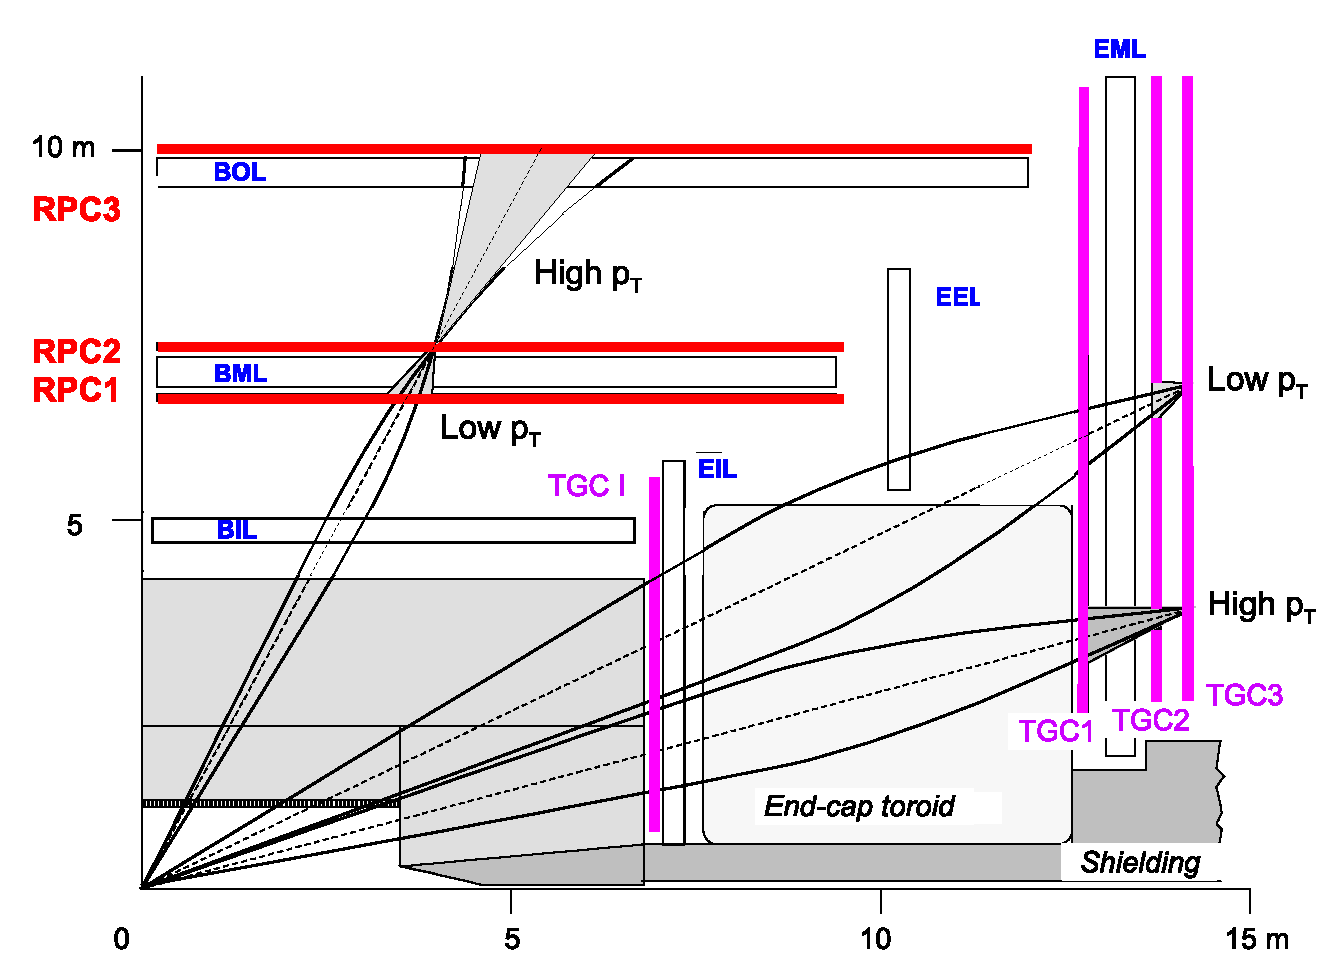
\includegraphics[width=0.75\textwidth, angle=0]{figures/LHC_ATLAS/RPC_TGC_schematics_5.eps}
\caption{ Schematic of the ATLAS muon trigger system.  The coincidence windows for muons of different $\pt$ is shown. (Figure taken from \cite{ATLAS_JINST}) \label{LHC:fig:MS_trigger}}
%\end{center}
\end{figure}
